\documentclass[a4j,twoside]{jarticle}
\usepackage[dvipdfmx]{graphicx, color}
\usepackage{float}
\usepackage{subcaption}
\usepackage{thesis_abst}
\usepackage{here}

\newcommand{\CONGEST}{\textsf{CONGEST}}
% 定理環境
\usepackage{amsthm} %定理用
\theoremstyle{definition}
\newtheorem{theorem}{定理}
\newtheorem{lemma}{補題}
\newtheorem{definition}{定義}
\newtheorem{fact}{事実}
\newtheorem*{prf*}{証明}

\addtolength{\oddsidemargin}{0mm}
\addtolength{\evensidemargin}{0mm}

\renewcommand{\baselinestretch}{1}

\種別{修 士}
\学籍番号{31414050}
\氏名{佐藤 僚祐}
\研究室{片山・金}
\系{ネットワーク}
\題目{$k$-独立点集合検証問題の分散計算複雑性}
\年度{2}

\begin{document}
\twocolumn[\vspace*{9mm}]
\begin{論文概要}
\setcounter{page}{1}


\section{研究背景}
分散グラフアルゴリズムとは,計算機を頂点,通信リンクを辺とみなしてネットワークをモデル化したグラフ上において,
そのネットワーク自身を入力として定義されるグラフアルゴリズム上の諸問題を解く枠組みである.本研究では,
分散アルゴリズムにおける代表的なモデルのひとつである{{\CONGEST}}モデルについて考える.
{\CONGEST}モデルにおいては,ある1つのノードにグラフ全体のトポロジの情報を集め,そのノード上で
逐次アルゴリズムを実行するという愚直なアプローチにより,任意の問題に対して自明に
$O (n^{2})$ラウンドの上界を得ることができる.従って,分散グラフアルゴリズムにおける複雑性について,
$\tilde{\Omega}(n^2)$ラウンドの下界を持つような問題は「最も難しい」問題ととらえることができる
\footnote{$\tilde{\Omega}(\cdot)$は,通常の$\Omega(\cdot)$記法から,
$\mathrm{polylog}(n)$の項を(相対的に十分小さい項として)無視した記法である.}.

本研究ではグラフ上の最適化問題の一つである,最大独立点集合問題に注目する.
逐次計算の文脈において,最大独立点集合問題はグラフ理論における重要な基本問題としてよく知られているが,
分散アルゴリズムの分野においても,同問題は一種の近傍頂点との間のリソース競合回避と見なすことができ,
数多くの応用が存在する.しかしながら,逐次計算の複雑性理論において,最大独立点集合問題は
NP完全であるのみならず,任意の定数$\epsilon > 0$に対して近似率$O(n^{1-\epsilon})$を達成不可能であることが
知られている\cite{haastad1999clique}ため,何らかの性能保証を持つ多項式時間アルゴリズムの設計は絶望的である.
一方で,分散アルゴリズムの分野においては,指数時間のローカル計算を許した{\CONGEST}モデルにおいて,
最大独立点集合問題の近似解を求めるためのラウンド複雑性が近年議論されており,上界,下界の両面から,
いくつかの結果が知られている.具体的には,{\CONGEST}モデルにおいて最大重み付き独立点集合の
$(1 + \epsilon) \cdot \Delta$-近似($\Delta$は頂点の最大次数) を高確率で
$\left(\mathrm{poly}(\log \log n)/\epsilon \right)$ラウンドで発見するアルゴリズム
\cite{kawarabayashi2019improved} や,最大独立点集合を発見するアルゴリズムに対する
$\Omega \left(\frac{n^{2}}{(\log n)^{2}}\right)$ラウンドの下界 \cite{censor2017quadratic},
最大独立点集合の$(\frac{3}{4} + \epsilon)$-近似を発見するアルゴリズムに対する
$\Omega \left(\frac{n^{2}}{(\log n)^{3}}\right)$ラウンドの下界 \cite{efron2020beyond} などが知られている.

本研究では,最大独立点集合計算の複雑性理解に対して,近似解アルゴリズムとは異なる面からのアプローチを試みる.
分散アルゴリズムにおける,上述の最大独立点集合問題の近似に関する議論は,本質的に指数時間のローカル計算を
許容したモデルを必要とするが,この仮定は必ずしも現実的とはいえない.そこで本研究では,近似解の分散計算複雑性ではなく,
(ある種の近傍の下での)局所最適解の複雑性に着目する.具体的には,$k$-極大独立点集合($k$-Maximal Independet Set, $k$-MIS,\cite{bollobas1991generalised})の発見問題に対する{\CONGEST}モデルでのラウンド複雑性を検討する.
逐次計算においては,単純な局所探索法で,$k=O(1)$に対して$k$-MISを多項式時間で計算することが可能であるため,
$k$-MISは多項式時間のローカル計算のみを許容する{\CONGEST}アルゴリズムにおいても取り扱うことが可能である.

自然な局所探索に基づいて$k$-MISを構成しようすると,与えられた独立点集合$I$が$k$-MIS,
つまり局所最適解かどうかを判定することが必要である.本研究ではこの判定問題($k$-MIS検証問題)に注目して,
{\CONGEST}モデル上のでのラウンド複雑性を検討する.

\section{本研究の成果}
{\CONGEST}モデルにおける$k$-MIS検証問題に関して,以下の結果が成立することを示した.
\begin{enumerate}
\item 1-MIS検証問題を$O(1)$ラウンドで解くアルゴリズムが存在する.
\item 2-MIS検証問題を解く任意のアルゴリズムの最悪時実行ラウンド数は$\tilde{\Omega} (\sqrt{n})$となる.
\item 3-MIS検証問題を解く任意のアルゴリズムの最悪時実行ラウンド数は$\tilde{\Omega}(n)$ラウンドとなる.
\item 任意の自然数$\ell \geq 1$に対して,$(4\ell + 5)$-MIS検証問題を解く任意のアルゴリズムの
最悪時実行ラウンド数は$\tilde{\Omega}\left((n^{2 - \frac{1}{\ell+1}})/\ell\right)$ラウンドとなる.
\end{enumerate}

上述する下界の証明はすべて,{\CONGEST}モデルでのラウンド数下界証明ための代表的な手法の一つである,
2者間通信複雑性における交叉判定問題からの帰着に基づいている.

\section{諸定義}
\subsection{{\CONGEST}モデル}
{\CONGEST}モデルにおいて,システムは単純無向連結グラフ$G =  (V,E)$により表現される.
ここで$V$はノードの集合で $|V| = n$とし, $E$は通信リンクの集合である.{\CONGEST}モデルでは
計算機は同期したラウンドに従って動作するものとする.
1ラウンド内で,隣接頂点へのメッセージ送信,隣接頂点からのメッセージ受信,内部計算を行う.各辺は単位ラウンドあたり
$b = O(\log n)$ビットを双方向に伝送可能であり,各ノードは同一ラウンドに異なる接続辺に異なるメッセージを
送信可能である.また,各ノードには$O(\log n)$ビットの整数値によるIDが付与されており,
自身の隣接ノードすべてのIDを既知であるとする.各ノードはグラフのトポロジに関する事前知識を持たないものとする.

\subsection{$k$-極大独立点集合}
\begin{definition}
頂点集合$I$に対して,以下を満たす頂点集合$I' \subseteq I$と$S\subseteq V \backslash I$のペアが
存在しないとき,$I$を$k$-極大独立点集合と呼ぶ.
\begin{enumerate}
\item $|I'| \leq k$
\item $|S| \geq |I'| + 1$
\item $(I \backslash I') \cup S$は独立点集合
\end{enumerate}
\end{definition}

\subsection{2者間通信複雑性}
2者間通信複雑性の枠組みでは,アリスとボブの二人のプレイヤーがそれぞれ$k$ビットの
0/1のデータ列で構成されるプライベートな入力$x$および$y$を持っているとする.
プレイヤーの目標は,結合関数$f(x,y)$をできるだけ少ない通信ビット数で計算する
ことである.また,アリスおよびボブは無限の計算能力を持つものとする.

2者間通信複雑性における重要な基本問題として,交叉判定問題(set-disjointness)がある.
この問題では,アリスとボブはそれぞれ$x \in \{0, 1\}^{k}$と$y \in \{0, 1\}^{k}$を入力として持ち,
目的は$\mathrm{DISJ}_{k} (x, y) :=\bigvee_{i = 1}^{k} x_{i} \land y_{i}$を計算することである.
$k$ビットの交叉判定問題を解くためにアリスとボブは通信によって$\Omega(k)$ビット交換する必要が
あることが知られており,この事実を用いて様々な下界の証明がされている.

\section{下界の証明の流れ}
本研究の下界の証明は下界グラフと呼ばれるグラフの構成法に基づく帰着手法を用いる.以下の条件を満たす下界グラフ$G^{x,y}=(V, E)$を構成する.
\begin{itemize}
\item $V$ はある互いに疎な頂点集合$V_A$,$V_B$に分割される.
\item $V_A$により誘導される部分グラフ$G_A$および$V_B$により誘導される部分グラフ$G_B$は
それぞれ入力文字列$x$および$y$のみに依存して決定される.
%\item $V_A$,$V_B$に対する頂点ラベリングの値はそれぞれ$x$,$y$のみに依存して決定される.
\item $G_A$と$G_B$の間にまたがるカット辺の集合$\mathit{Cut}$は$x$および$y$いずれの値にも
依存しない.
\item $G^{x,y}$は$\mathrm{DISJ}_{k} (x, y)=1$のときかつそのときのみある特性$P$を持つ.
\end{itemize}
グラフ$G^{x, y}$の構造の概要を図 \ref{Gxy} に示す.
\begin{figure}[ht]
\begin{center}
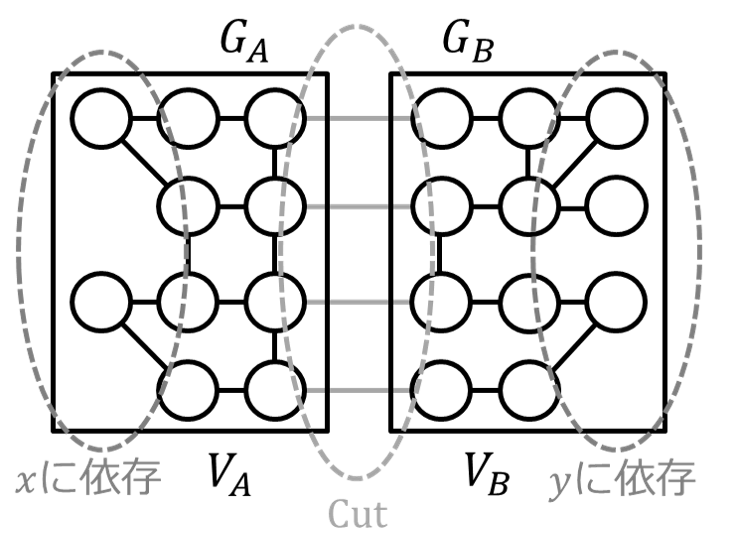
\includegraphics[width=40mm]{Gxy.png}
\end{center}
\caption{$G^{x, y} = (V, E)$}
\label{Gxy}
\end{figure}

アリスとボブは構成した下界グラフ上で特性$P$を判定する{\CONGEST}アルゴリズム$\mathcal{A}$の実行をシミュレートする.
アリスは$V_{A}$中の頂点,ボブは$V_{B}$中の頂点のシミュレートを担当する.
$G_{A}$中の辺で送信されるメッセージ,あるいは$G_{B}$中の辺で送信されるメッセージは,
アリスとボブがそれぞれ通信なしに計算できるため,それとカット辺$\mathit{Cut}$を通じて送信されるメッセージを互いに受信できれば,
$G^{x,y}$全体での$\mathcal{A}$のシミュレーションを(アリスとボブが手分けして)実行することができる.
今アルゴリズム$\mathcal{A}$が$r$ラウンドで終了するとすると,
アリスとボブは上述のシミュレーションにより特性$P$の判定結果を知ることが可能であり,
それに必要な通信ビット数は$O(r \cdot |\mathit{Cut}| \cdot \log n)$ビットである.
下界グラフの構成より,特性$P$の真偽と$x$,$y$が交叉しているかどうかの真偽は対応するため,
このシミュレーションは$O(r \cdot |\mathit{Cut}| \cdot \log n)$ビットの通信量で交叉判定問題$(x,y)$を解いている.
$k$ビットの交叉判定問題を解くため必要な通信量は$\Omega(k)$であり,
これより$r = \Omega (k / |\mathit{Cut}| \cdot \log n)$の下界を得ることができる.

本研究では$k=2, 3, 4\ell(\ell \geq 1)$それぞれに対して「$\mathrm{DISJ}_{k} (x, y)=1$のときかつそのときのみ
$G^{x,y}$中に与えられている独立点集合が$k$-MISでない」という特性$P_{k}$を持つよう下界グラフ$G_{x,y}$の構成法を提案し,その正当性を証明した.
\section{まとめと今後の課題}
本研究では,{\CONGEST}モデルにおける$k$-極大独立集合検証問題の計算複雑性を示した.$k=4, \ldots, 8$については
現在$k=3$と同じ下界しか得られていないため,このギャップを埋められるかが今後の課題である.

\bibliographystyle{plain}
\bibliography{M2sato_abst}

\clearpage
\end{論文概要}
\end{document}
